%%%%%%%%%%%%%%%%%%%%%%%%%%%%%%%%%%%%%%%%
%% MCM/ICM LaTeX Template %%
%% 2024 MCM/ICM           %%
%%%%%%%%%%%%%%%%%%%%%%%%%%%%%%%%%%%%%%%%
\documentclass[12pt]{article}
\usepackage{geometry}
\geometry{left=1in,right=0.75in,top=1in,bottom=1in}

%%%%%%%%%%%%%%%%%%%%%%%%%%%%%%%%%%%%%%%%
% Replace ABCDEF in the next line with your chosen problem
% and replace 1111111 with your Team Control Number
\newcommand{\Problem}{A}
\newcommand{\Team}{2403424}
%%%%%%%%%%%%%%%%%%%%%%%%%%%%%%%%%%%%%%%%

\usepackage{newtxtext}
\usepackage{amsmath,amssymb,amsthm}
\usepackage{newtxmath} % must come after amsXXX
\usepackage{cite}
\usepackage{graphicx}
\usepackage{xcolor}
\usepackage{fancyhdr}
\usepackage{listings}
\usepackage{xeCJK}
\definecolor{codegreen}{rgb}{0,0.6,0}
\definecolor{codegray}{rgb}{0.5,0.5,0.5}
\definecolor{codepurple}{rgb}{0.58,0,0.82}
\definecolor{backcolour}{rgb}{0.95,0.95,0.92}

\lstdefinestyle{mystyle}{
    backgroundcolor=\color{backcolour},   
    commentstyle=\color{codegreen},
    keywordstyle=\color{magenta},
    numberstyle=\tiny\color{codegray},
    stringstyle=\color{codepurple},
    basicstyle=\ttfamily\footnotesize,
    breakatwhitespace=false,         
    breaklines=true,                 
    captionpos=b,                    
    keepspaces=true,                 
    numbers=left,                    
    numbersep=5pt,                  
    showspaces=false,                
    showstringspaces=false,
    showtabs=false,                  
    tabsize=2
}

\lstset{style=mystyle}

\lhead{Team \Team}
\rhead{}
\cfoot{}

\newtheorem{theorem}{Theorem}
\newtheorem{corollary}[theorem]{Corollary}
\newtheorem{lemma}[theorem]{Lemma}
\newtheorem{definition}{Definition}
%%%%%%%%%%%%%%%%%%%%%%%%%%%%%%%%
\begin{document}
\graphicspath{{.}}  % Place your graphic files in the same directory as your main document
\DeclareGraphicsExtensions{.pdf, .jpg, .tif, .png}
\thispagestyle{empty}
\vspace*{-16ex}
\centerline{\begin{tabular}{*3{c}}
		\parbox[t]{0.3\linewidth}{\begin{center}\textbf{Problem Chosen}\\ \Large \textcolor{red}{\Problem}\end{center}}
		 & \parbox[t]{0.3\linewidth}{\begin{center}\textbf{2024\\ MCM/ICM\\ Summary Sheet}\end{center}}
		 & \parbox[t]{0.3\linewidth}{\begin{center}\textbf{Team Control Number}\\ \Large \textcolor{red}{\Team}\end{center}} \\
		\hline
	\end{tabular}}
%%%%%%%%%%% Begin Summary %%%%%%%%%%%
% Enter your summary here replacing the (red) text
% Replace the text from here ...
\begin{center}
	\textbf{\Huge Lamprey: A New Model for the Spread of an Invasive Species}
	\begin{figure}[h]
		\centering
		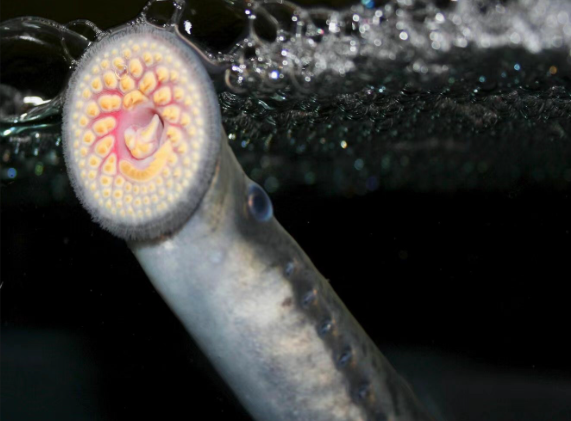
\includegraphics[width=0.7\textwidth]{LampreyFigure.png}
		\caption{Lamprey by Great Lakes Science Center\cite{sea-lamprey-2}.}
	\end{figure}
	% real summary beginning
\end{center}
As a powerful invasive species in the Great Lakes from the 1940s, lamprey populations are closely linked to the entire Great Lakes ecosystem. The female propotion of lampreys is positively correlated with the growth rate in their larval stages, and the growth rate of these larvae is affected by the amount of available food resources. The purpose of this study was to establish an analytical model to simulate the reproductive activities of lampreys under the influence of sex ratio changes and to evaluate the impact of sex ratio change mechanisms on lamprey offspring. We also build models of interactions between lampreys and other species to analyze the relationship between lamprey population development and ecosystems. \newline
In the study, we used a total of three models; \\
\textbf{Model 1}: Lotka-Volterra model that introduced gender change factors;\\
\textbf{Model 2}: Lamprey's body shape-first mate selection strategy and reproduction model;\\
\textbf{Model 3}: Based on the multi-species Lotka-Volterra model Matrix iteration model. \\We hope this study will help optimize the control of lampreys in the Great Lakes, and provide assistance in studying the reproductive activities of lamprey populations. 
% to here
%%%%%%%%%%% End Summary %%%%%%%%%%%
\newpage
\tableofcontents
\newpage
%%%%%%%%%%%%%%%%%%%%%%%%%%%%%%
\clearpage
\pagestyle{fancy}
% Uncomment the next line to generate a Table of Contents
%\tableofcontents 
\newpage
\setcounter{page}{1}
\rhead{Page \thepage\ }
%%%%%%%%%%%%%%%%%%%%%%%%%%%%%%


%%%%%%%%%%%%%%%%%%%%%%%%%%%%%%
\section{Introduction}
\subsection{Problem Background}
Sea lampreys in the Great Lakes region exhibit sex ratio variation that adapts to environmental conditions. 
The Great Lakes ecosystem has observed fluctuations in lamprey populations, with the sex ratio influenced by 
the growth rates during their larval phase, which are contingent upon food availability. In environments with 
limited food, a slower growth rate skews the population toward a higher male ratio up to 78\%. Conversely, with 
better food availability, the male percentage decreases to approximately 56\%. The sex ratio adaptation in sea 
lampreys affects prey species, predator populations, and competition dynamics within the Great Lakes. The ability 
to adjust sex ratios allows lampreys to potentially stabilize their population in varying conditions, influencing 
the broader ecosystem balance.
\subsection{Q4}
\section{Further Research}

\section{Conclusion}
\newpage
%Appendices 
\newpage
\listoffigures
\listoftables
\bibliography{library,images}
\bibliographystyle{plain}
\newpage
\section*{Appendices}
\subsection*{Program for Q1}
\lstinputlisting[language=Python]{../Src/Q1.py}
\lstinputlisting[language=Python]{../Src/Q1_2.py}
\subsection*{Program for Q2}
\lstinputlisting[language=Python]{../Src/Q2_1.py}
\lstinputlisting[language=Python]{../Src/Q2_2.py}
\lstinputlisting[language=Python]{../Src/Q2_3.py}
\subsection*{Program for Q3, Q4}
\lstinputlisting[language=Python]{../Src/Q3-Q4.py}
%%%%%%%%%%%%%%%%%%%%%%%%%%%%%%
\end{document}
